\documentclass[11pt,space]{ctexart} 
\usepackage{GEEexam_Verbal_Passage}

\usepackage{tabularx}

\newcommand{\note}[1]{\noindent {\heiti\textbf{注\hspace{1em}}}#1.}

\usepackage{tikz}
\renewcommand{\oval}{
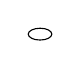
\begin{tikzpicture}
  \draw (0,0) ellipse (.15cm and .075cm);
\end{tikzpicture}
}

\newcommand{\choices}[5]{%
    \ifx\relax#4\relax % 检查第四个参数是否未定义（即\relax）
        % 如果第四个参数未定义，创建一个三参数的表格
        \begin{center}
        \begin{tabularx}{\linewidth}{>{\raggedleft\arraybackslash}p{0.03\linewidth} p{0.9\linewidth}}
            $\square$ & {#1} \\
            $\square$ & {#2} \\
            $\square$ & {#3} 
        \end{tabularx}
        \end{center}
    \else % 如果第四个参数已定义，创建一个五参数的表格
        \begin{center}
        \begin{tabularx}{\linewidth}{>{\raggedleft\arraybackslash}p{0.03\linewidth} p{0.9\linewidth}}
            \oval & {#1} \\
            \oval & {#2} \\
            \oval & {#3} \\
            \oval & {#4} \\
            \oval & {#5} 
        \end{tabularx}
        \end{center}
    \fi
}

\newcommand{\passage}[2]{
\begin{multicols}{2}
\noindent {#1}
\columnbreak % 列的分隔符

\noindent {#2}
\end{multicols}
}


\usepackage{multicol}
\usepackage{lipsum}

\begin{document}

\section*{主旨题}

\passage{Many theorists now doubt that heat loss from Earth's core and radioactive decay are sufficient by themselves to produce all the energy driving the tectonic plates whose movements have helped shaped Earth's surface. This leaves a loose end in current geological theory. Herbert Shaw argues that because scientists have underestimated the input of substantial amounts of energy from extraterrestrial impactors (asteroids and comets striking Earth), they have difficulty accounting for the difference between the quantity of energy produced from sources intrinsic to Earth and that involved in plate tectonics. Whereas most geologists have treated the addition of energy through the bombardment of Earth's surface by such impactors as a process separate and independent from the movement of Earth's tectonic plates, Shaw asserts that these processes are indivisible. Shaw's revolutionary "open-system" view recognizes a continuum between terrestrial and extraterrestrial dynamics, whereas modern plate tectonic theory, like the classical geology developed during the nineteenth century, is founded on the view that Earth's geological features have changed through gradual, regular processes intrinsic to Earth, without reference to unique catastrophic events. Classical geology borrowed a decisive, if unspoken, premise from Newton-the independence of Earth's processes from any astronomical context.
}{The author's primary purpose is to
\choices{
identify the influences informing a particular geological theory about the processes that have shaped Earth's surface.
}{
identify differences between two views of the extraterrestrial impactors and argue that the phenomenon has influenced the development of plate tectonic theory.
}{
argue that an explanation is based on dubious evidence and propose an alternative explanation.
}{
discuss an explanation and place that explanation under theoretical context.
}{
suggest that apparent discrepancy poses a serious problem for a particular theory that many have believed.
}
}
\note{
这题容易错选E，但要注意E只有概括文段的前一半，文段的后一半在说这种新的解释如何行得通，也穿插着两个理论的对比以及部分理论假设的细节，因此还是D最合适
}

\newpage
\passage{In The Life of Charlotte Bronte(1857), the first and the most celebrated biography of novelist Charlotte Bronte, Elizabeth Gaskell promoted the long-persisting romantic view of Bronte as having no connection with the rest of English society at a time when industrialization was causing much turbulence, but as having sprung naturally, like so much purple heather, out of the English countryside. Gaskell also portrayed Bronte as irreproachably proper, incapable of "unladylike" feelings or dangerous views; this was at variance with the subversive spirit Matthew Arnold accurately discerned, albeit with distance, deep within Bronte` s fiction. While correcting many of Gaskell` s errors and omissions at last, even Winifred Gerin` s Charlotte Bronte: The Evolution of Genius (1967) failed to discard Gaskell` s viewpoint. Feminists have introduced new interpretations of Bronte` s life, but it is primarily Juliet Barker who takes into account the larger world that impinged on that life - the changing England in which old divisions of class and gender were under pressure.
}{The primary purpose of the passage is to
\choices{
consider similarities in several studies of Charlotte Bronte' s life.
}{
defend a particular view of Charlotte Bronte's life,
}{
discuss a change in perspective on Charlotte Bronte' s life.
}{
depict the social environment in which Charlotte Bronte lived.
}{
portray Charlotte Bronte as an early feminist writer.
}
}
\note{
文中列举了多人对于Charlotte Bronte的生活的描述方式，然而作者比较认同的是最先的那个版本。其实从最开始到倒数第二句话都很难明确区分出作者是在defend还是在discuss changes，而最后一句话比较明显，明显偏向陈述新的沿革。区分B和C的另一个方法是，作者并不是在辩护关于Charlotte Bronte的生活的某一观点，而是为某一叙事方式背书，所以B不够准确
}

\newpage
\passage{In \textit{A Raisin in the Sun}, Lorraine Hansberry does not reject integration or the economic and moral promise of the American dream; rather, she remains loyal to this dream while looking, realistically, at its incomplete realization. Once we recognize this dual vision, we can accept the play's ironic nuances as deliberate social commentaries by Hansberry rather than as the “unintentional” irony that Bigsby attributes to the work. Indeed, a curiously persistent refusal to credit Hansberry with a capacity for intentional irony has led some critics to interpret the play's thematic conflicts as mere confusion, contradiction, or eclecticism. Isaacs, for example, cannot easily reconcile Hansberry's intense concern for her race with her ideal of human reconciliation. But the play's complex view of Black self-esteem and human solidarity as compatible is no more “contradictory” than Du Bois' famous, well-considered ideal of ethnic self-awareness coexisting with human unity, or Fanon's emphasis on an ideal internationalism that also accommodates national identities and roles.
}{The author's primary purpose in the passage is to
\choices{
explain some critics' refusal to consider \textit{Raisin in the Sun} a deliberately ironic play.
}{
analyze the fundamental dramatic conflicts in \textit{Raisin in the Sun}.
}{
affirm the thematic coherence underlying \textit{Raisin in the Sun}.
}{
...
}{
...
}

\noindent It can be inferred from the passage that the author believes which of the following about Hansberry's use of irony in \textit{Raisin in the Sun}?
\choices{
It reflects Hansberry's reservations about the extent to which the American dream has been realized.
}{
It is justified by Hansberry's loyalty to a favorable depiction of American life.
}{It shows in the play's thematic conflicts.}{}{}
}
\note{
文段在反驳中说明了\textit{Raisin in the Sun}的主题，是有意为之的冲突，批驳了认为它混乱的观点。第一题需要高级的同义转述，"affirm the thematic coherence"其实就和文中为\textit{Raisin in the Sun}主题的统一性辩护是一致的意思。至于A，行文思路更多是在边立边破，而不是先破后立。

第二题的AB选项由第一句话得出，Hansberry对于American dream是持一定保留态度的，也没有提到"favorable depiction"。C项需要看懂作者的立场和作者批驳的声音；没理解\textit{Raisin in the Sun}的人认为文中的"thematic conflicts"就是完全的混乱，而作者是在批驳这些观点而强调\textit{Raisin in the Sun}的内部主题的连贯性，所以这正说明了Hansberry用到的讽刺是故意地体现在"thematic conflicts"内的
}

\newpage
\section*{目的题}
\passage{Although some \textbf{skeptics} point to Arctic places such as the high latitudes of Greenland, where temperatures seem to have fallen, a recent scientific report concludes that in recent decades average temperatures have increased faster in the Arctic than elsewhere. Scientists have long suspected that several factors lead to greater temperature swings at Earth's polar regions than elsewhere. First, most of the Arctic is covered in snow and ice, which are highly reflective; if snow and ice melt, the exposed soil, which absorbs heat, serves to accelerate warming. Second, the polar atmosphere is thin, so little energy is required to warm it. Third, less solar energy is lost in evaporation at the frigid poles than in the tropics.
}{In pointing to the apparent temperature change in the high latitudes of Greenland, the \textbf{skeptics} mentioned in the passage intend to raise as a question whether
\choices{
Greenland is less likely to experience extreme temperature changes than are other areas of the Arctic.
}{
Those more localized temperature drops might indicate an important trend not captured by the upward trend of average Arctic temperatures.
}{
There might be a reversal of the temperature trend in the high latitudes of Greenland.
}{
The factors that cause temperature change in the high latitudes of Greenland are different from those that affect the rest of the Arctic.
}{
Greenland has more ice and snow on the ground than do other areas of the Arctic.
}
}
\note{
文段中说的结论是南极洲地区的气温上升得比全球其他地方都快，并分析了背后的原因。skeptics的立场自然是怀疑这个结论的正确性，他们指出南极洲部分地区（即"high latitudes of Greenland"）的气温升高来表示怀疑，本质上就是不认可文中的结论。如果再进一步往深了说就是，认为局地的气温变化反而暗示了整体气温上升趋势所不能包含的信息，从而以"high latitudes of Greenland"作为挑战结论的证据。注意C选项缩小了讨论范围，skeptics援引"high latitudes of Greenland"并不单纯是为了争在那儿有不同的趋势。A选项可能是正确的，但和主旨其实无关，也不会是skeptics的目的。同理，D选项可能是对的，但skeptics质疑的是结论的正确性，不会转变为对结论成立背后可能的原因的挑战
}

\newpage
\section*{逻辑题}

\passage{New methods developed in genetic research have led taxonomists to revise their views on the evolutionary relationships between many species. Traditionally the relatedness of species has been ascertained by a close comparison of their anatomy. The new methods infer the closeness of any two species' relationship to each other directly from similarities between the species' genetic codes.
}{Which of the following conclusions is best supported by the information?
\choices{The apparent degree of relatedness of some species, as determined by anatomical criteria, is not borne out by their degree of genetic similarity.}{When they know the differences between two species' genetic codes, taxonomists can infer what the observable anatomical differences between those species must be.}{The degree to which individuals of the same species are anatomically similar is determined more by their genetic codes than by such environmental factors as food supply.}{...}{...}
}
\note{
阅读理解一定要忠于原文，非必要不要加上自己的理解（即引入额外的信息）。GRE中很常见关于因素或时间顺序的对比和陈列，但只要文中没有直接的对比，都不要主观推测，相关的选项大多是错的。

文中介绍了关于物种进化的观点的改进，但并没有说传统的就是不好的，更新的就是更优越的。C选项甚至引入了无关的环境因素，必不选。原文的逻辑是，物种之间的相近程度在传统方法是由解剖学决定的，而新的思路增加了由基因相似性推测物种亲缘的方法（是推测而不是决定），但这不能推导出基因相似性能推断解剖学上的差异，B错误；不过这也说明了由解剖学决定的亲缘关系可能不会由基因相似性证实，A涉及了细致的推理和同义转述，bear out意为“证实”
}

\passage{The damage that trucks do to highways escalates dramatically with the weight borne per axle. New regulations increase the maximum permitted vehicle weight; these regulations will therefore allow onto the highway trucks capable of doing even more damage than those currently permitted.
}{The argument is open up to criticism on the grounds that it
\choices{
fails to establish that the level of damage done by trucks is a serious problem.
}{
omits evidence about one of the two relevant factors.
}{
ignores the possibility that careful driving can lessen damage to highways.
}{
presumes that trucks are the only vehicles capable of causing substantial damage to highways.
}{
presumes that something is bound to happen just because it is allowed to happen.
}
}

\note{文章说到卡车对于高速路的损坏取决于每个轮子的承重，也就是说总重和轮子数量这两个因素共同决定。反对新规的理由只有提到重量会增加，而没有提到轮子数量的事儿。可能的反驳是，卡车的重量增加通常也伴随着轮子数的增加，对高速路的损害不见得更大，因此选B}

\passage{A law has been proposed requiring the cargo boxes of trucks carrying gravel to be covered by a tarpaulin, because vehicles driving close behind open-topped gravel trucks can be damaged by gravel flying off these trucks. The law is unlikely to substantially reduce such damage, however: flying gravel is much less likely to come from the cargo box itself than from the grooves of the tires, in which gravel can become wedged during loading.
}{Which of the following, if true, provides the strongest support for the argument given?
\choices{
The drivers of vehicles behind a gravel truck are more likely to remain close behind the truck if the trucks cargo box is covered than if it is uncovered.
}{
Most trucks that carry gravel already carry tarpaulins that their drivers use to cover the cargo box when they are carrying sand, which can blow out of the cargo box in significant quantities.
}{
Of all the damage that occurs to vehicles on the highway, debris that flies off trucks is the cause of only a very small fraction.
}{
The proposed law allows open-topped trucks on the highway to have uncovered cargo boxes whenever their cargo boxes are empty.
}{
Because of the great weight of a load of gravel, the driver of a gravel truck is often driving much more slowly than most of the other vehicles on the road.
}
}
\note{
原文其实是分析了造成损失的两个可能原因，一个是伤害值小的来自cargo boxes，另一个是伤害值大的来自tires。该法案只是消除了伤害值小的源头，而没有改善tires带来的伤害，所以颁布了也不会带来显著的减少。要想加强原文的结论，可以是放大伤害值大的部分的影响，或者削弱伤害值小的部分的作用。

A选项合理。加盖帆布之后，后续续车辆更可能靠近运输石子的卡车，从而更容易受到轮胎里飞出的碎石造成的伤害，伤害不会减少，甚至还可能增加，加强了原文结论。BDE都是明显的无关选项。C选项最有迷惑性。注意关注点在于法案能否减少石子的伤害，这和石子的伤害占各种伤害的比例无关；无论比例大小如何，这都无法左右这个结论，因为其他种类的damage并不是本文讨论对象（注意"gravel flying off trucks"包含从boxes飞出来的也包括从tires飞出来的，不要主观臆断地认为只有前者进而理解错选项）
}


\passage{Electric washing machines, first introduced in the United States in 1925, significantly reduced the amount of time spent washing a given amount of clothes, yet the average amount of time households spent washing clothes increased after 1925. This increase is partially accounted for by the fact that many urban households had previously sent their clothes to professional laundries. But the average amount of time spent washing clothes also increased for rural households with no access to professional laundries.
}{Which of the following, if true, most helps to explain why the time spent washing clothes increased in rural areas?
\choices{
People with access to an electric washing machine typically wore their clothes many fewer times before washing them than did people without access to electric washing machines.
}{
...
}{
...
}{
...
}{
...
}
}
\note{
文中并没有假设electronic washing machine在农村和城市的普及差异，不要带入主观理解胡乱臆测。根据题意，城市和农村的差别只在于前者有professional laundries而后者没有。前者的洗衣时间增加可以理解，（一部分原因）是从professional laundries到每家每户的electronic washing machine，规模经济消失了。而后者洗衣时间依旧增加，理论上没有这一规模经济消失的因素，那么必然有更强大的因素推高了洗衣时间，选项中选和professional laundries以及electronic washing machine普及率城乡差异无关的选项即可
}

\passage{Newspaper Editorial: 

Last year, Mayor Stephens established a special law-enforcement task force with the avowed mission of eradicating corruption in city government. The mayor's handpicked task force has now begun prosecuting a dozen city officials. Since all of these officials were appointed by Mayor Bixby, Mayor Stephens' predecessor and longtime political foe, it is clear that those being prosecuted have been targeted because of their political affiliations.
}{Which of the following, if true, most weakens the editorial's argument?
\choices{
Almost all of the officials who have served in city government for any length of time are appointees of Mayor Bixby.
}{
All of the members of the anticorruption task force had other jobs in city government before the task force was formed.
}{
Former mayor Bixby did not publicly oppose Mayor Stephens' establishment of the anticorruption task force.
}{
...
}{
...
}
}
\note{
读完文段之后最先想到的反驳文中观点的论据就是，那些被抓贪腐的官员也有一些新市长的人马，或者抓贪腐的官员不乏前市长的人。选项AB需要钻研细节：A选项不是直接说反腐官员是前市长任命的，但文段中说这些人马来自市政府，其实也间接说明了反腐力量就是前市长当时任命的；B选项只是说反腐官员之前就有任职，但没有准确说这个“之前”是什么时候，不能说就是前市长任期内就已经上任了，因此B选项不充分。C选项是最弱的，这从情理上能削弱论断，但和文中的逻辑链条无关，不到最后不要选
}

\newpage
\section*{细节题}

\passage{Most popularizations of science actually do more harm than good. Why? The single most important feature of scientific work is not this or that specific result. Instead, what science accomplishes--and what physics in particular accomplishes so beautifully--is the linking of diverse phenomena, the binding together of a myriad of predictions and explanations. What nearly all popularizations do is systematically undermine the progressive reasoning that links principles, conventions, experiments, and laws. Bad science writing splinters the most interesting feature of science, its long run of connected argumentation, into isolated metaphors that last just long enough to evoke a particular result: black holes are said to be huge funnels and quantum electron orbits are characterized as diffuse clouds.
}{The passage implies that most popular science writing
\choices{
focuses on discrete results arrived at by scientific reasoning
}{
spends more time describing scientific personalities than scientific processes
}{
gives readers an incomplete view of the interrelatedness of scientific discovery
}
{
...
}
{
...
}
}
\note{
A选项对应"popularizations do is systematically undermine the progressive reasoning that links principles, conventions, experiments, and laws"，同义转述为"discrete results"。B选项对应"Bad science writing splinters the most interesting feature of science, its long run of connected argumentation【对应scientific processes】, into isolated metaphors【对应scientific personalities（特点）】"；这边的同义转化比较隐晦，"isolated metaphors"自然是用比喻的手法形象地把一些科学结果展现给读者，是对特征的描述和强调。C即文段大意
}

\passage{In recent decades, scholars of American literature have skillfully revealed authors' simultaneous accommodation and resistance to an increasingly commercialized, capitalized environment during the early nineteenth century. Historians of the period have not, however, fully exploited literary criticism, due to the disciplinary boundaries that mark contemporary academic research. Few historians have extensive training in critical theory and its specialized languages, and the sheer volume of work in early American history and literature challenges anyone who would master either field, much less both. Moreover, historians study people across the nation, but much literary scholarship called “American” actually examines works produced in northeastern states. And historians usually study the operations of capitalism in its details, while literary critics produce a generalized picture of literary commodification.
}{The passage cites which of the following as a reason for historians' failure to fully exploit literary criticism?
\choices{
historians' overly thematic approach to literature
}{
historians' conservative notion of what constitutes literature
}{
historian's lack of interest in critical theory
}{
the distinctive nature of much literary criticism
}{
the ahistorical quality of much literary criticism
}
}
\note{
B选项擅自对于学科的分野加了"conservative"的描述，这容易因为主观理解误选，不要认为学科的领域有局限就说这样的边界是保守的（大的原则还是一致的，就是忠于原文，不要加入个人理解）。D和E有一些相似之处，但不能说literary criticism有一些非历史研究的因素就不能被历史学家理解，这一点在文中没有提及，并且也不是主要因素。D其实是对原文"disciplinary boundaries"的高级转述
}

\passage{There is mounting evidence that the frequency and magnitude of landsliding is changing in many parts of the world in response to climate change. This is not surprising, given that precipitation is one of the two external triggering mechanisms--the other being seismic activity--involved in the formation of landslides. Evidence from the past clearly indicates that cycles of elevated landslide activity have been followed by cycles of low activity, and that these are correlated with climate fluctuations over a variety of timescales. What sets current changes in landslide activity apart is the likely influence of anthropogenic [i.e., human-caused] factors, either acting alone or in concert with climate, which can further modify the process of landsliding and the nature of ecosystem responses. Among these factors, deforestation and land-use change have the potential to influence the frequency and magnitude of landsliding because of their direct effects on vegetation attributes that influence slope stability. The extent and conditions under which mountain ecosystems are resilient to these changes--that is, the amount of disturbance they can absorb before changing into states with different structure and function--are not known. Addressing this issue is crucial for the long-term conservation of mountainscapes.
}{The passage makes which of the following claims?
\choices{
A rise in precipitation resulting from human factors has increased the frequency and magnitude of landsliding.
}{
Human factors have led to greater changes in landsliding activity than have cyclical climate fluctuations.
}{
Decreases in landsliding activity have historically been accompanied by changes in climate.
}{
Slope stability is more influenced by seismic activity than it is by human factors.
}{
Changes in land-use patterns in mountain ecosystems are generally correlated with changes in climate.
}
}
\note{文中并没有比较因素之间的重要性，尽管单独指出了人类因素，但也不能说明人类因素就胜过其他因素，尤其是不要带入个人的理解。C选项定位到原文为“cycles of elevated landslide activity have been followed by cycles of low activity, and that these are correlated with climate fluctuations over a variety of timescales”，注意这里用了很微妙的同义转述，关于"cycles of elevated landslide activity"只说它"decrease"的一半，而把"correlate with"也变成了"accompanied by"}

\newpage
\passage{According to Hill and Spicer, the term "nation-state” is a misnomer, since the ideal model of a monolingual, culturally homogeneous state has never existed, not even among Europeans, who invented the nation-state concept and introduced it to the rest of the world. Modern European states, they argue, emerged after the Renaissance through the rise of nations (i.e., specific ethnic groups) to positions of political and economic dominance over a number of other ethnic groups within the bounded political territories. The term "nation-state”, Hill and Spicer argue, obscures the internal cultural and linguistic diversity of states that could more accurately be called "conquest states.” The resurgence of multiple ethnic groups within a single state, Hill says, is not "potentially threatening to the sovereign jurisdiction of the state,” as Urban and Sherzer suggest; rather, the assertion of cultural differences threatens to reveal ethnocentric beliefs and practices upon which conquest states were historically founded and thus to open up the possibility for a "nation-state” in which conquered ethnic groups enjoy equal rights with the conquering ethnic group but do not face the threat of persecution or cultural assimilation into the dominant ethnic group.
}{According to the passage, Hill and Spicer define nations as which of the following?
\choices{
Coalitions of distinct ethnic groups with similar concerns.
}{
Distinct ethnic groups.
}{
Culturally homogeneous states.
}{
Linguistically diverse states.
}{
Territorially bounded states.
}
}
\note{
无论如何必须要找到Hill and Spicer表达观点的叙述，这边的定位比较精巧，"Modern European states, they argue, emerged after the Renaissance through the rise of nations \textbf{(i.e., specific ethnic groups)} to positions of political and economic dominance over ..."。Distinct除了“清楚的，独特的”外还有“不同的”的意思，在这里就和原文的"specific"相对应。注意D和E选项只是nations的特点，而不是nations的定义
}

\newpage
\passage{Historian Colin Calloway argues that in the late colonial period preceding the American Revolution (1775-1783), the British government sought to seal off territory west of the Appalachian Mountain from the encroachment of land-hungry White settlers, to negotiate with Native American peoples as independent foreign states, and to guarantee the integrity of traditional native American hunting grounds. By contrast, White Americans, released by the outbreak of the Revolution from the constraints of Britain's allegedly benevolent policies, are portrayed by Calloway as ruthless land-grabbers whose new national government endorsed their rapacity. Bernard Bailyn argues, however, that the "Americans" who encroached on Native American land during the Revolution had been British only a few years before. When, during and after the Revolution, White Americans seized Native American land by any available means, they were continuing a tradition dating back to the earliest years of English settlement in North America. And, according to Bailyn, the British government's prewar efforts to preserve the trans-Appalachian west for Native Americans resulted not from humanitarian virtue or ethnic tolerance but from British Merchants' desire to maintain their lucrative trade with native Americans and the government' s desire to control immigration and avoid costly conflict between White and Native Americans over land.
}{It can be inferred that both Bailyn and Calloway would probably agree with which of the following assertions regarding the relations between White Americans and Native Americans concerning the trans-Appalachian west?
\choices{
The American Revolution unleashed an unprecedented wave of expropriation of Native American land by White settlers.
}{
The British government's prewar policy towards the Native Americans was determined largely by the interests of British merchants who traded with the Native Americans.
}{
The British government tried to keep White settlers out of the trans-Appalachian west primarily in order to prevent disputes over land between those settlers and Native Americans.
}{
The new national colonial government to negotiate with Native American peoples as independent foreign states.
}{
One objective of the British government's land policy prior to the American revolution was to prevent White settlers from moving to the western side of the Appalachian Mountains.
}
}
\note{问共同点的题一定要自己先有答案再去看选项，否则只会思绪变得更混乱。在文章方面也要先理清文章的结构，然后寻找策略。比如这篇文章就是一半一半地阐述两边的观点，那就是分别总结然后找交集；有的文章有偏向或者侧重，那么就从文章的叙述或概括中直接找到答案}

\newpage
\passage{A divide between aesthetic and technical considerations has played a crucial role in mapmaking and cartographic scholarship. Since nineteenth century cartographers, for instance, understood themselves as technicians who did not care about visual effects, while others saw themselves as landscape painters. That dichotomy structured the discipline of the history of cartography. Until the 1980s, in what Blakemore and Harley called "the 'Old is Beautiful' paradigm," scholars largely focused on maps made before 1800, marveling at their beauty and sometimes regretting the decline of the pre-technical age. Early mapmaking was considered art while modern cartography was located within the realm of engineering utility. Alpers, however, has argued that this boundary would have puzzled mapmakers in the seventeenth century, because they considered themselves to be visual engineers.
}{According to the passage, Alpers would say that the assumptions underlying the "paradigm" were
\choices{
inconsistent with the way some mapmakers prior to 1800 understand their own work.
}{
unconcerned with the difference between the aesthetic and technical questions of mapmaking.
}{
insensitive to divisions among cartographers working in the period after 1800.
}{
...
}{
...
}
\noindent It can be inferred from the passage that, beginning in the 1980s, historians of cartography
\choices{
placed greater emphasis on the beauty of maps made after 1800.
}{
expanded their range of study to include more material created after 1800.
}{
came to see the visual details of maps as aesthetic objects rather than practical cartographic aids.
}{
reduced the attention they paid to the technical aspects of mapmaking.
}{
...
}
}
\note{
第一题，由“paradigm”定位原文，可知该观点强调艺术性。由Alpers定位最后一句，17世纪的制图者并不存在美学和技术的分水岭，17世纪的制图者们认为自己既考虑美学因素也考虑了技术因素。

第二题，文章里交代的是20世纪80年代之前的状况，题干问的是20世纪80年代之后的情况。原文的"until"暗示了"until"后陈述的内容只到1980s之前，之后就变化了；因此这题考查取反逻辑，时间互相取反，那么句子里的动作也应当同时取反。再结合句内提到学者们开始注意到1800年以前的地图非常精美，有艺术成就，那么我们合理推断他们是有对照物的，才能得出前者更美的结论。因此答案选B。
}



\newpage
\section*{推断题}

\passage{Availability and management of water greatly influenced human settlement in the Maya Lowlands, and much of Mayan social innovation was centered on storing excess water for times of need. In northern Yucatan the permanent water table is sufficiently shallow that it can be accessed by natural wells known as cenotes. However, over much of the Maya Lowlands, the water table is too deep to have been available to the Maya. In response, ...
}{The passage suggests which of the following about cenotes?
\choices{
They allowed people in northern Yucatan to avoid dependence on artificial reservoirs.
}{
They were less capacious than the artificial reservoirs found in the Maya Lowlands.
}{
They helped protect people in the Maya Lowlands from prolonged droughts.
}{
They allowed the Maya to store excess water for times of need.
}{
They were an important Mayan social innovation.
}
}
\note{
不要看到主旨句之后就认为后面的内容全在主旨句的意思统领下，在进入最核心的阐述之前，完全可能会有适度的铺垫和对比。比如本文的第一句就是主旨句，但northern Yucatan明显不是讲人们关于获取水的创新（不要理解为这一句提到的"cenotes"就是"Mayan social innovation"），甚至衬托了"However"之后的核心
}

\passage{Unlike the static, classically composed portraits produced by her mentor Walker Evans, twentieth-century New York photographer Helen Levitt's photographs seem candid and spontaneous. Whereas Evans' subjects look directly into the camera, so that photographer and subject conspire in the making of a portrait, Levitt's subjects seem caught unawares. As a “street” photographer, before the term's invention, Levitt has claimed to have attempted to capture life as she found it. But there is a paradox to her technique. Her off-the-cuff aesthetic seemingly guarantees objectivity, since she was recording street scenes she happened upon, yet her photographs could be said to be highly subjective, to be reflections of Levitt's own distinctive preoccupations and ways of seeing. Unlike Evans' images, Levitt's are solely the products of the photographer without the conscious participation of their subjects. The repetitions evident in Levitt's choices of subjects, for example, her many photographs of children in masks and disguises, reveal more about Levitt herself than about those subjects.
}{The passage suggests which of the following about street photography?
\choices{
It characteristically depicts groups of people rather than individual subjects.
}{
It tends to depict a narrow and repetitious range of subject matter.
}{
It creates the impression of spontaneity but often actually involves scenes contrived by the photographer.
}{
Its early practitioners were not accorded much recognition for their aesthetic achievements.
}{
It had not been named as such when Levitt began practicing this kind of photography.
}
}
\note{
大多数的文字都在说Levitt的风格和实践，不能完全和street photography画等号，比如BC选项都是陷阱。一定要定位到提到了street photography的语句，尽管有的成分在句子中并不突出。这里要选E，应为原文"As a 'street' photographer, before the term's invention, Levitt has claimed ..."，说明Levitt的实践是开拓性的。GRE的很多推断题都是从不起眼的细节设置考点
}

\passage{David Belasco's 1912 Broadway production of The Governor's Lady created a sensation with a scene set in a Childs cafeteria, a chain restaurant that was an innovator in food standardization and emblematic of modern everyday life. While Belasco's meticulously detailed reproduction of an immediately recognizable setting impressed the public, it was derided by progressive theater critics who championed the New Stagecraft theories of European artists like Max Reinhardt. The New Stagecraft rejected theatrical literalism; it drew inspiration from the subjectivity and minimalism of modern painters, advocating simplified sets designed to express a dramatic text's central ideas. Such critics considered Belasco a craftsman who merely captured surface realities: a true artist eliminated the inessential to create more meaningful, expressive stage images.
}{It can be inferred that the theater critics would be most likely to agree with which of the following statements about the theatrical productions?
\choices{
Theatrical productions that seek to eliminate the inessential also often eliminate theatrical elements that enhance the expressiveness of a play.
}{
Theatrical productions that faithfully recreate the visual details of everyday life are unlikely to do justice to a good play's central ideas.
}{
Theatrical productions that employ the minimalism characteristic of modern paintings may have greater appeal to modern audiences than productions that rely on theatrical literalism.
}{
...
}{
...
}
}
\note{
通常推断题要对原文中给的信息进行取反或者给出必要条件。注意GRE的一些表述，尤其是取反之后的，可能会显得绝对或换一些不确定是否忠于原文的表述，但如果没有明显的偷换概念，就要大胆选。

这边的线索在于"The New Stagecraft rejected theatrical literalism;  ..., advocating simplified sets designed to express a dramatic text's central ideas."取反，就知道这一派会认为如果所有都极力刻画细节，那么就无法很好地呈现中心思想。注意尽管这一派坚持“大道至简”，但这不代表他们就认为“大道至简”的效果就会比“忠于现实”的更好——GRE的经验是，只要文段没有给出观点/效果/情感等的对比，就不要妄自带入经验下结论
}

\passage{Historian F. W. Maitland observed that legal documents are the best — indeed, often the only—available evidence about the economic and social history of a given period. Why, then, has it taken so long for historians to focus systematically on the civil (noncriminal) law of early modern (sixteenth- to eighteenth-century) England? Maitland offered one reason: the subject requires researchers to "master an extremely formal system of pleading and procedure." Yet the complexities that confront those who would study such materials are not wholly different from those recently surmounted by historians of criminal law in England during the same period. Another possible explanation ...
}{The passage suggests that the history of criminal law in early modern England differs from the history of civil law during that same period in that the history of criminal law 
\choices{
is of more intellectual interest to historians and their readers.
}{
has been studied more thoroughly by historians.
}{
is more relevant to general social history.
}{
involves the study of a larger proportion of the population.
}{
does not require the mastery of an extremely formal system of procedures.
}
}
\note{
定位到原文是"Yet the complexities that confront those who would study such materials are not wholly different from those recently surmounted by historians of criminal law in England during the same period."这一句，注意第一个"those"是指研究civil law的历史学家（后面的定语从句说明了），第二个"those"是指"the complexities"，这样后面的"surmounted by historians of criminal law"才说得通。这说明history of criminal law的困难已经被征服了，换个高级的表述就是这已经被更透彻地研究了
}

\passage{Early scholars described square dances as a type of ancient English country dance carried to the southern Appalachian Mountains and preserved unchanged for generations. However, while the Appalachian fiddle repertoire does include traditional reels that can be traced back to the British Isles, it also includes breakdowns, rags, and other musical features native to America. Appalachian songs similarly range from British ballads to African American blues. Given this musical diversity-not to mention the iconic presence of the banjo, an instrument with African roots-it would be naive to think the accompanying dances are purely English forms. While sections of Appalachia are relatively isolated, trade, travel, and immigration have continually introduced new cultural elements, including innovations in social dances, into the region's rural traditions.
}{Based on the passage, it can be inferred that Appalachian square dancing
\choices{
is a much younger tradition than scholars once believed.
}{
has evolved significantly compared to its original form.
}{
has introduced novel elements to English country dancing.
}{
was not traditionally accompanied by breakdowns or rags.
}{
probably did not contribute to the development of blues music.
}
}
\note{
推断题的很多细节是在对比中给出的，而呈现在句子中可能就是一些作为补充的定语或者同位语，这里定位到"However, while the Appalachian fiddle repertoire does include ..., it also includes breakdowns, rags, ..."

注意不要选B选项，尽管Appalachian square dancing加入了很多本土化的元素，不能就此下结论"has evolved significantly"。这种结论性质的判断、以及比较关系必须要忠于原文，如果没有直接陈述，不要凭借主观臆断选
}

\newpage
\passage{Eighteenth-century women played a significant part in British political life. Up and down the social scale they performed a variety of political acts, everything from purchasing political artifacts such at plates, handkerchiefs, and fans to penning political pamphlets, starring in civic processions, sponsoring boycotts, arguing over public issues in their own debating societies, rioting, and uttering seditious words. Whereas historians used to see female political involvement in this century as isolated or aberrant, they now stress the continuity and normalcy of such activity, especially for aristocratic women. Given the familial nature of aristocratic politics, noble women were actually expected to act as political advisors and agent for their husbands, to canvass in elections, to serve as political hostesses, to seek and dispense political patronage. They did so routinely long before the eighteenth and deep into the nineteenth century. Patrician women had such far-reaching political influence, it has been argued recently, that they actually stood to rise by expansion of the electorate to include women. Fruitful as this new historiography has been, however, it has politics and its inattention to ideology. Given the widespread political activity of women, why expansion of suffrage did not happen in the eighteenth-century?
}{The author would most likely agree with which of the following statements about political acts performed by eighteenth-century women?
\choices{
They had little influence on the outcome of elections.
}{
They were aimed largely at the expansion of the electorate.
}{
They probably were discouraged by men with political aspirations.
}{
They represented a new development in British society.
}{
They were sometimes perceived as being negative.
}
}
\note{
前面都在说18世纪的女性在政治相关活动中的积极参与，但最关键的还是"However"后的转折。最后三句话，以反问的方式表达了即使这些女性为何这样积极参与政治活动，但还是不能为她们自己赢得选举权，直接得出推论她们还是对选举结果的影响微乎其微
}

\newpage
\passage{The physicist Wallace Sabine pioneered the scientific study of architectural acoustics when he was asked in 1895 to fix a university lecture hall in which the echo of a speaker's words rendered them unintelligible. He found that the length of time it takes a sound's echo to decay is determined by the absorption of the sound's original energy by surrounding material. By hanging panels of sound-absorbing felt on the walls, Sabine reduced the echo enough to make the hall usable. And the data he compiled yielded a mathematical formula for the relationship between a room's echo duration, its quantity and quality of sound-absorbing materials, and its spatial volume.
}{The passage suggests that Sabine's work made which of the following possible for the first time?
\choices{
to make a room soundproof
}{
to build an auditorium out of sound-absorbing materials
}{
to construct an enclosed space in which sound would not echo
}{
to design a building to meet predetermined specifications with regard to echo duration
}{
to render any large room usable for public lectures and performances
}
}
\note{
A偷换概念，Sabine的工作是减弱、吸收回声，从而使礼堂达到“可使用”的状态，而不是使得房子“隔音”；B偷换概念，文章只说Sabine使用吸音板解决了该礼堂的回音问题，不是说Sabine第一次用吸音材料建了房子；C偷换概念，只是“吸收回声”，不是“不产生回音”；E说的“让任何大房间都可以用于演讲、表演”，未提及，扩大范围。D的正确性要用到推理，也就是Sabine用数学公式刻画了消减回声的规律，这可以作为未来设计满足特定回声要求的建筑物（文中的例子本身不能说明D对，因为Sabine面临的不是"predetermined specification"）
}


\newpage
\section*{词义题}

\passage{Although vastly popular during its time, much nineteenth-century women`s fiction in the United States went unread by the twentieth-century educated elite, who were taught to ignore it as didactic. However, American literature has a tradition of didacticism going back to its Puritan roots, shifting over time from sermons and poetic transcripts into novels, which proved to be perfect vehicles for \textbf{conveying} social values. ...
}{In the context in which it appears, "conveying" most nearly means
\choices{
carrying.
}{
transferring.
}{
granting.
}{
imparting.
}{
projecting.
}
}
\note{
文中的"conveying"有“传授，诉说”之意，故不仅仅有“传递”的基础含义，还有一些说教的意蕴在内。carrying只有“携带”之意，甚至不能如transferring完美表达“传递”之意，但二者都没有像imparting那样表露出“教导，启发”的意思。另外，impart knowledge/value/...是固定用法
}

\passage{Among academics involved in the study of Northern Renaissance prints (reproducible graphic artworks), an orthodox position can be said to have emerged. This position regards Renaissance prints as \textbf{passive} representations of their time — documents that reliably record contemporary events, opinions, and beliefs — and therefore as an important means of accessing the popular contemporary consciousness. In contrast, pioneering studies such as those by Scribner and Moxey take a strikingly different approach, according to which Northern Renaissance prints were purposeful, active, and important shaping forces in the communities that produced them. ...}{Replacement of the word "passive" with which of the following words results in the least change in meaning for the passage?
\choices{disinterested}{submissive}{flaccid}{supine}{unreceptive}
}
\note{
字面意义上passive和submissive最相近，但这边的意思更接近说Renaissance prints是记录这个时代元素的工具，工具本身是没有携带主观性的，因此选disinterested
}

\newpage
\passage{Many paleontologists have linked the origin of the vertebrate skeleton to the need for defense. According to this hypothesis, the first, soft-bodied vertebrates, living in the seas of the Cambrian period, began to evolve extensive coverings of bony scales or plates as the result of predation by numerous invertebrate carnivores. Teeth are thought to have been secondary features evolved over millions of years from those plates that had migrated to the mouth. Another hypothesis, however, contends that many of the definitive characteristics of vertebrates, such as paired eyes, would not have evolved unless the first vertebrates were predatory.
}{In the context in which it appears, "contends" most nearly means
\choices{
competes
}{
disputes
}{
maintains
}{
demonstrates
}{
struggles
}
}
\note{
这边看似强调观点对比，实际上更中立一些的话则还是单纯作为对立观点的陈述；实际上，contend只有“认为，坚持”的意思，而没有“争辩”之意。另外，dispute that后跟的是争辩的观点，而不是己方的对立观点
}

\passage{Data of modern and historic peasant communities suggest that individuals and communities specialize in ceramic production for trade primarily to offset subsistence shortfalls arising from inadequate or insufficient agricultural land. Harry investigated whether this correlation of ceramic specialization with agricultural \textbf{marginality} occurred among prehistoric inhabitants of the American Southwest. At Arizona's West Branch site, occupied A. D. 900-1100, abundant pottery manufacturing materials suggest villagewide ceramic production in excess of that needed for household purposes.
}{Replacement of the word “\textbf{marginality}” with which of the following words results in the least change in meaning for the passage?
\choices{
peculiarity
}{
insignificant
}{
nonconformity
}{
deficiency
}{
futility
}
}
\note{
词义题中，词语的原义切记只能作为参考，更多的时候要“忘记”词的本意，更多考虑其在文本中的特定含义，尤其是注意和前后文一些词语基于对比/同义等关系的呼应。这里的"marginality"就和前文的"shortfalls"呼应，指的是农业收入的不稳定性
}

\end{document}